\chapter{Configuración y resultados del entrenamiento final}
\label{cap:AnexoH}

Este anexo documenta los hiperparámetros del modelo desplegado en producción y los resultados de evaluación obtenidos en los conjuntos de validación y prueba de CodiEsp~\cite{miranda2020}.

\section{Modelo base}

Se emplea \texttt{IIC/RigoBERTa-Clinical}~\cite{garciasubies2026rigobertaclinical}, variante clínica de RigoBERTa~\cite{vacaserrano2022rigoberta} basada en la arquitectura XLM-RoBERTa-large. La ventana de contexto nativa del modelo es de 512 \emph{tokens}, que es también la longitud máxima empleada en entrenamiento e inferencia.

\section{Hiperparámetros}

La Tabla~\ref{tab:hyperparams} recoge la configuración de la ejecución de producción (\texttt{20260530T030233Z}, paso~36).

\begin{table}[h]
\centering
\caption{Hiperparámetros del entrenamiento final.}
\label{tab:hyperparams}
\begin{tabular}{lll}
\hline
\textbf{Parámetro} & \textbf{Valor} & \textbf{Descripción} \\
\hline
\multicolumn{3}{l}{\textit{Datos}} \\
\texttt{num\_codes}      & 1767          & Clases (códigos CIE-10 completos presentes en CodiEsp) \\
\texttt{max\_length}     & 512           & Longitud máxima de secuencia en \emph{tokens} \\
\texttt{full\_codes}     & \texttt{True} & Granularidad completa (p.\,ej.\ \texttt{E11.9}), sin truncar a 3~caracteres \\
\hline
\multicolumn{3}{l}{\textit{Optimización}} \\
\texttt{lr}              & $10^{-4}$     & Tasa de aprendizaje \\
\texttt{warmup\_ratio}   & 0{,}1         & Fracción de pasos de calentamiento \\
\texttt{lr\_schedule}    & plateau       & Reducción al detectar estancamiento en val. F1 \\
\texttt{weight\_decay}   & 0{,}1         & Regularización L2 \\
\texttt{epochs\_max}     & 150           & Máximo de épocas permitido \\
\texttt{epochs\_run}     & 150           & Épocas ejecutadas (alcanzó el máximo sin parada temprana) \\
\texttt{patience}        & 20            & Épocas sin mejora antes de parar \\
\hline
\multicolumn{3}{l}{\textit{Arquitectura}} \\
\texttt{dropout}         & 0{,}3         & \emph{Dropout} en la cabeza de clasificación \\
\texttt{freeze\_layers}  & 20            & Capas del \emph{encoder} congeladas al inicio \\
\texttt{unfreeze\_every} & 30            & Épocas entre descongelaciones \\
\texttt{unfreeze\_layers}& 4             & Capas descongeladas en cada paso \\
\texttt{unfreeze\_lr\_ratio} & 0{,}1     & Factor de reducción de LR para capas descongeladas \\
\hline
\multicolumn{3}{l}{\textit{Función de pérdida}} \\
\texttt{label\_smoothing} & 0{,}1       & Suavizado de etiquetas \\
\texttt{pos\_weight\_cap} & 10{,}0      & Peso máximo de la clase positiva (desequilibrio) \\
\hline
\multicolumn{3}{l}{\textit{Batch}} \\
\texttt{batch\_size}     & 8             & Tamaño de mini-lote efectivo en GPU \\
\texttt{grad\_accum}     & 4             & Pasos de acumulación de gradiente \\
\texttt{effective\_batch}& 32            & Tamaño de lote efectivo resultante \\
\hline
\multicolumn{3}{l}{\textit{Inferencia}} \\
\texttt{threshold}       & 0{,}3         & Umbral de probabilidad para activar una etiqueta \\
\texttt{pretrain\_epochs}& 10            & Épocas de precalentamiento con todo congelado \\
\texttt{attn\_impl}     & \texttt{flash\_attention\_2} & Implementación de atención (FlashAttention 2) \\
\hline
\end{tabular}
\end{table}

\section{Resultados de evaluación}

El sistema emplea dos estrategias de umbral diferentes. Durante el entrenamiento se usa un umbral global fijo para monitorizar la mejora. También se evaluaron umbrales por clase optimizados sobre el conjunto de validación, que ajustan individualmente el punto de corte de cada uno de los 1.767 códigos; se descartaron para producción por sobreajustar la validación (véase más abajo).

La Tabla~\ref{tab:final-results} muestra ambas métricas para el modelo de producción (ejecución \texttt{20260530T030233Z}, paso~36).

\begin{table}[h]
\centering
\caption{Resultados del modelo final (paso~36) en validación y prueba, por estrategia de umbral.}
\label{tab:final-results}
\begin{tabular}{llrrl}
\hline
\textbf{Conjunto} & \textbf{Umbral} & \textbf{F1-micro} & \textbf{F1-macro} & \textbf{MAP} \\
\hline
Validación & global 0,3 & 0{,}4945 & 0{,}119 & 0{,}544$^{r}$ \\
Validación & por clase  & 0{,}551  & 0{,}152 & n/d \\
Test       & global 0,3 & 0{,}4887 & 0{,}109 & \textbf{0{,}437}$^{g}$ / 0{,}537$^{r}$ \\
Test       & por clase  & 0{,}468  & 0{,}113 & n/d \\
\hline
\end{tabular}

\smallskip\par\footnotesize $^{g}$~MAP sobre el gold completo (directamente comparable con el \emph{benchmark} CodiEsp). $^{r}$~MAP restringido a los 1.767 códigos del vocabulario del modelo. Los umbrales por clase se ajustan sobre validación y sobreajustan (F1-micro 0,551 en validación frente a 0,468 en prueba), por lo que la configuración de producción emplea el umbral global de 0,3.
\end{table}

La ejecución seleccionada como referencia de evaluación en profundidad es \texttt{20260530T030233Z} (paso~36). La política de despliegue en producción es dinámica (se detalla en el capítulo de Desarrollo, Anexo~\ref{cap:AnexoF}); esta ejecución fue, en su momento, la mejor de las registradas hasta ese punto. Con umbral global de 0,3 alcanza F1-micro = 0{,}4945 en validación y 0{,}4887 en prueba. Los umbrales por clase optimizados sobre validación llegan a F1-micro = 0{,}551, pero sobreajustan (0{,}468 en prueba), por lo que producción emplea el umbral global. El MAP por documento sobre el conjunto de prueba (métrica oficial del \emph{benchmark} CodiEsp) es \textbf{0{,}437} sobre el gold completo (0{,}537 restringido al vocabulario del modelo), situándose dentro del rango del \emph{benchmark}~\cite{miranda2020}, por detrás de los \emph{ensembles} y diccionarios de las primeras posiciones. El \emph{recall} de 0,458 debe leerse contra el techo de 0,825 que impone el vocabulario del modelo (497 de los 2.842 pares del \emph{gold} de prueba son códigos que no aparecen en entrenamiento): supone el 55,5\,\% del máximo alcanzable.

\paragraph{Procedencia de las cifras.} Las métricas de esta tabla proceden de dos pasadas de evaluación distintas: el barrido de umbral y el MAP de prueba se calculan con \texttt{eval\_test.py}, mientras que las cifras de validación reportadas como referencia del paso~36 provienen del registro de entrenamiento. Ambas difieren en la tercera cifra decimal (por ejemplo, F1-micro de validación 0,4945 frente a 0,4933, o MAP de prueba 0,4373 frente a 0,4342) porque la inferencia de una de ellas se realiza con precisión reducida. La diferencia no altera ninguna conclusión, pero conviene declararla para que el lector no la interprete como una inconsistencia.

La diferencia entre F1-micro y F1-macro refleja el fuerte desequilibrio de clases del corpus: el modelo rinde bien sobre los códigos frecuentes, pero tiene dificultades con los poco representados. Este es un límite inherente al corpus de entrenamiento de 500 documentos, donde la mayoría de los 1.767 códigos aparecen menos de cinco veces.

\section{Curvas de entrenamiento}

La Figura~\ref{fig:epochs-graph} muestra la evolución del F1-micro de validación y la pérdida de entrenamiento a lo largo de las épocas para los \emph{runs} realizados con \texttt{IIC/RigoBERTa-Clinical}.

\begin{figure}[h]
\centering
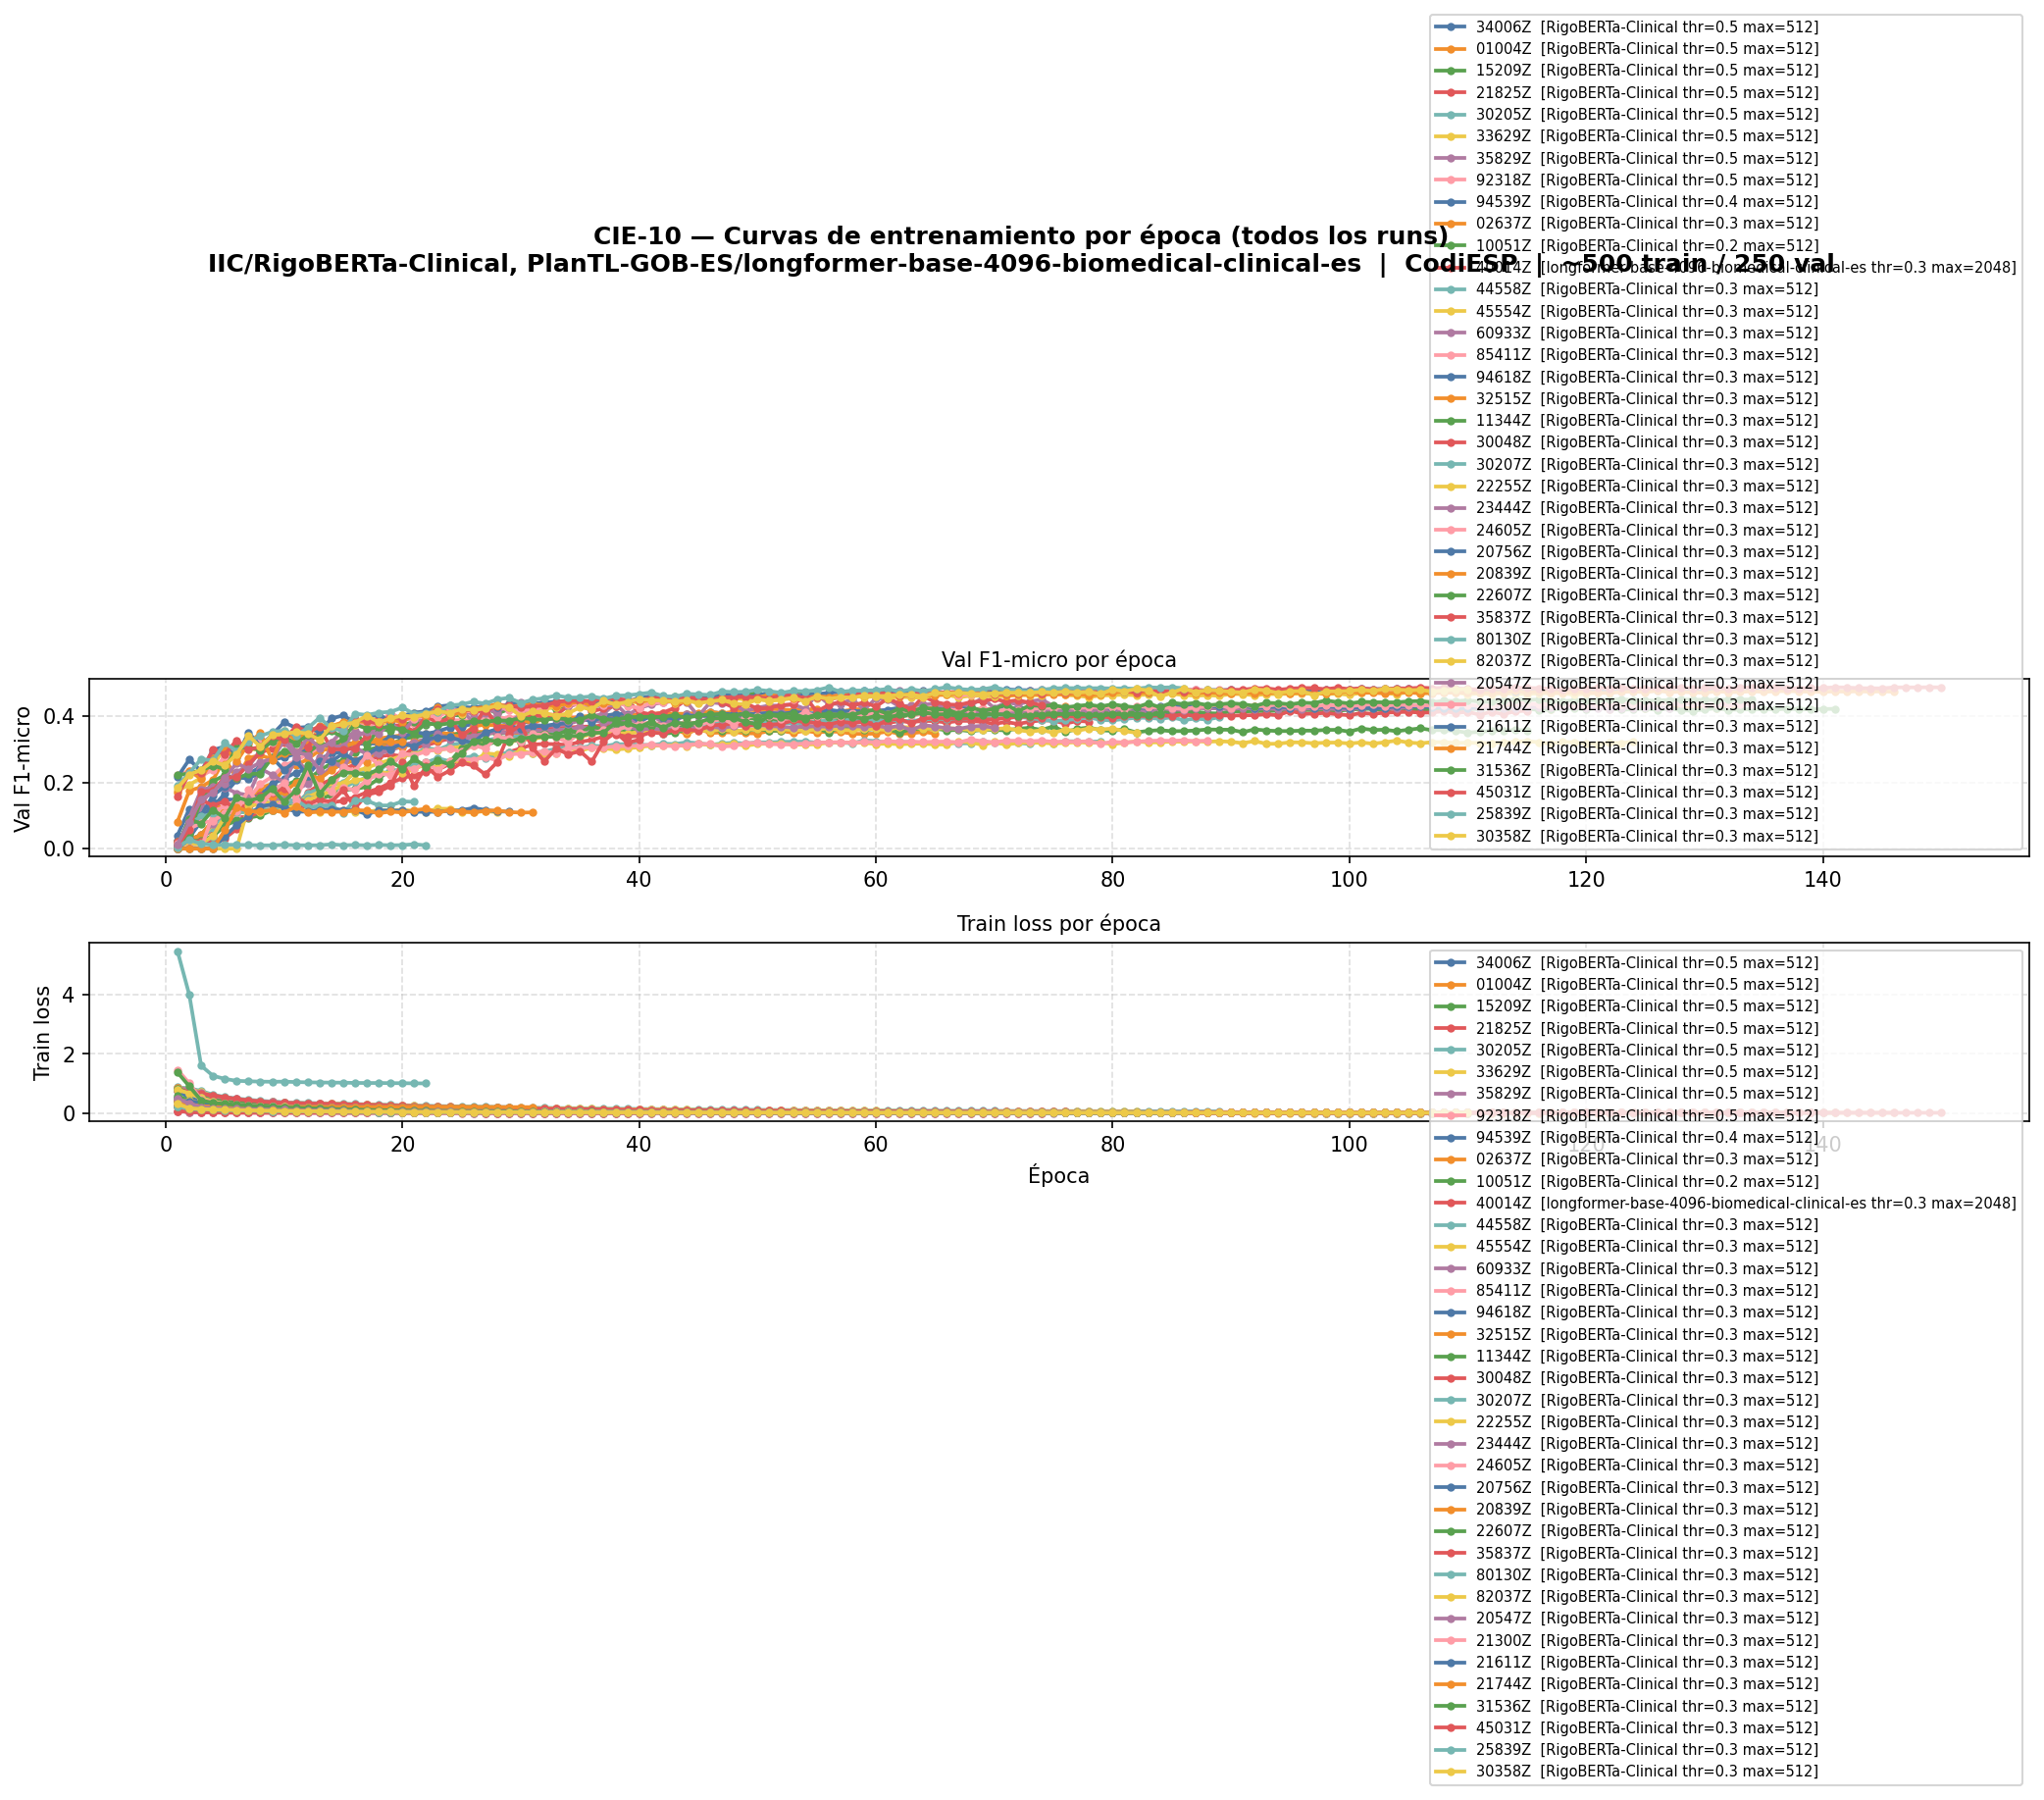
\includegraphics[width=\textwidth]{figs/all_epochs_graph}
\caption{Curvas de entrenamiento: F1-micro de validación y pérdida de entrenamiento por época.}
\label{fig:epochs-graph}
\end{figure}

\section{Artefactos del modelo}

Los artefactos del modelo desplegado en producción se encuentran en \texttt{ai\_engine/model/}:

\begin{description}
    \item[\texttt{classifier.pt}] Pesos del modelo PyTorch (ejecución del paso~36).
    \item[\texttt{thresholds.json}] Umbrales por clase optimizados sobre el conjunto de validación.
    \item[\texttt{config.json}] Metadatos del modelo activo: nombre, fichero de pesos, fichero de umbrales y parámetros de inferencia.
\end{description}
